\section{Referencia del Archivo /media/docs/progra/c++/compiladores1/proy2/godzilla/src/parserheader.h}
\label{parserheader_8h}\index{/media/docs/progra/c++/compiladores1/proy2/godzilla/src/parserheader.h@{/media/docs/progra/c++/compiladores1/proy2/godzilla/src/parserheader.h}}
interfaz entre el GUI y el parser. 



Este gr\'{a}fico muestra que archivos directa o indirectamente incluyen a este archivo:\begin{figure}[H]
\begin{center}
\leavevmode
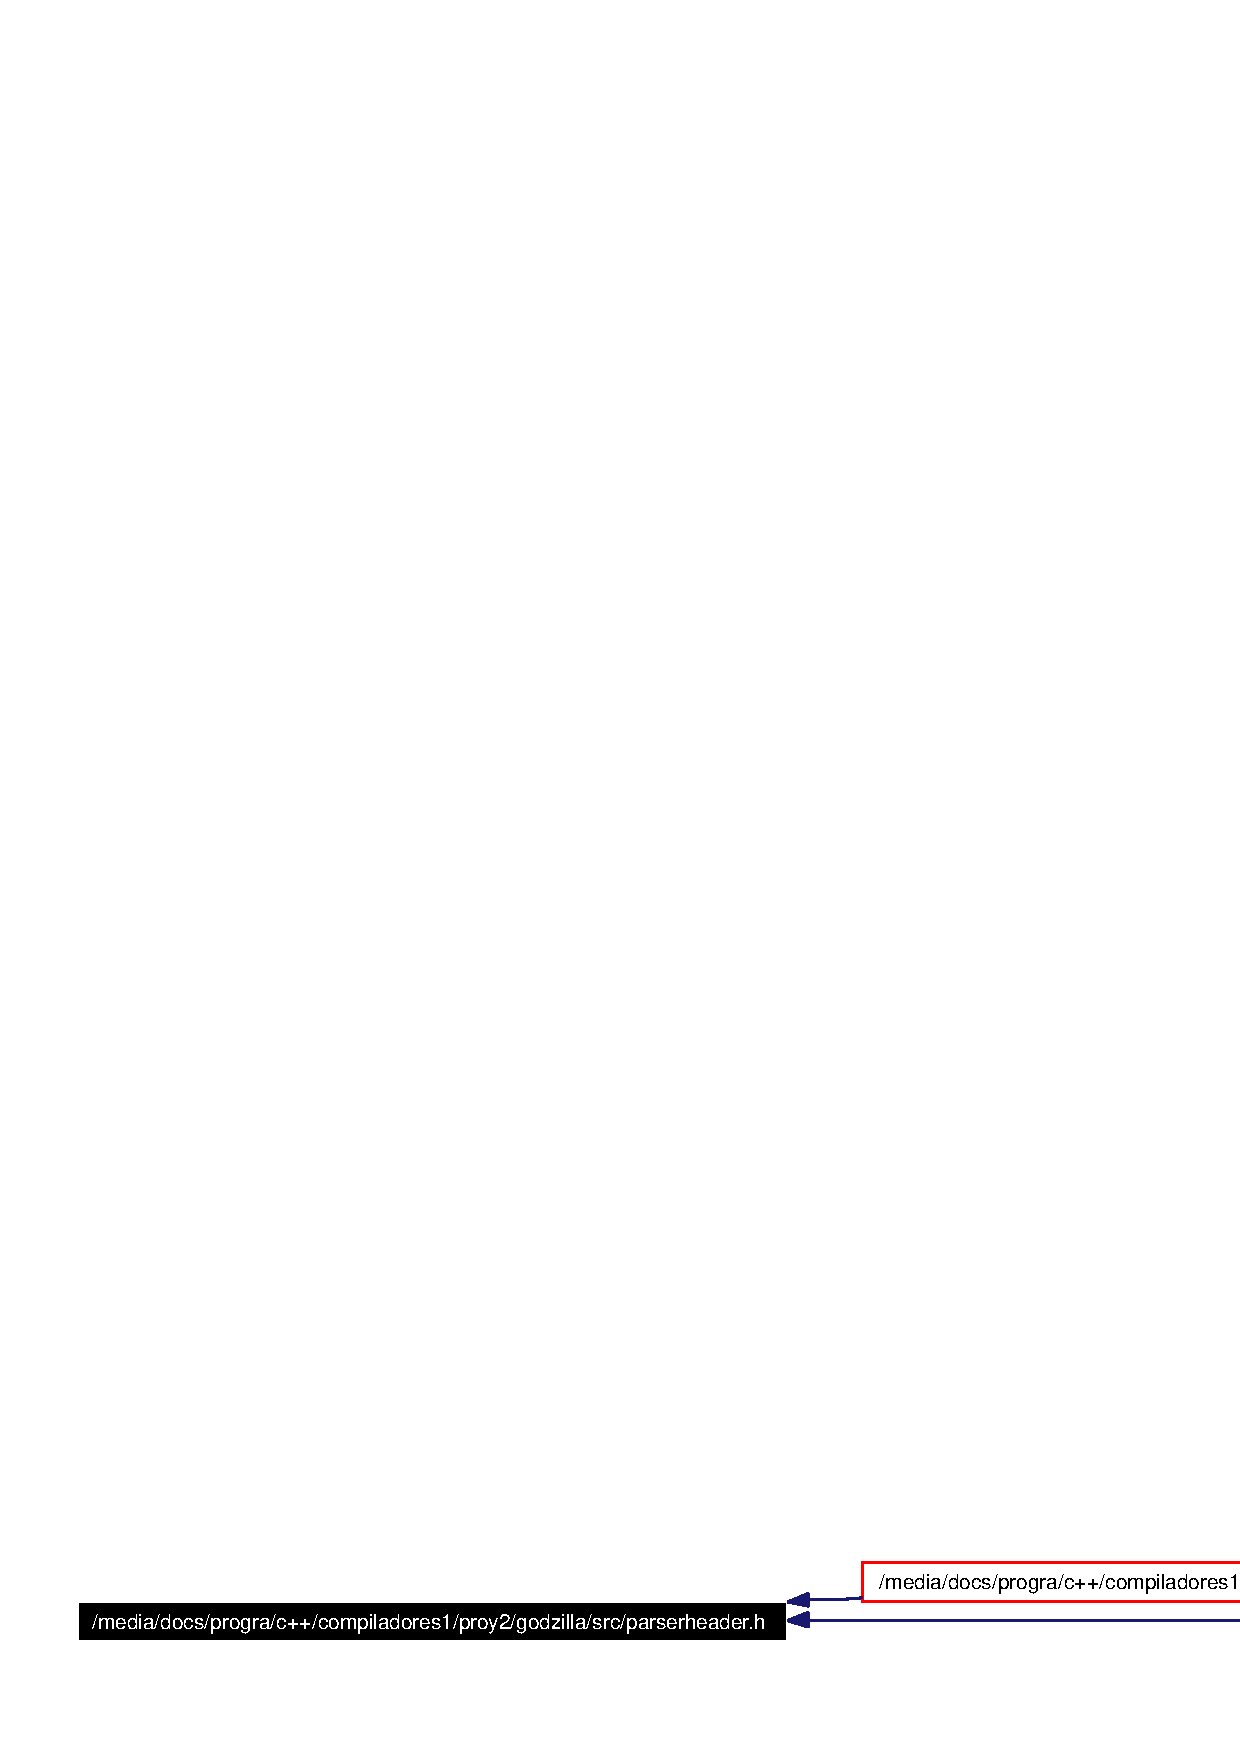
\includegraphics[width=420pt]{parserheader_8h__dep__incl}
\end{center}
\end{figure}
\subsection*{Funciones}
\begin{CompactItemize}
\item 
int {\bf inputparse} (const char $\ast$filein, const char $\ast$fileout)
\begin{CompactList}\small\item\em Interfaz para parser y lexer. \item\end{CompactList}\item 
int {\bf generar\-Salida\-Error} (const char $\ast$fileerr)
\begin{CompactList}\small\item\em Interfaz para colaerr. \item\end{CompactList}\end{CompactItemize}


\subsection{Descripci\'{o}n detallada}
interfaz entre el GUI y el parser. 



Definici\'{o}n en el archivo {\bf parserheader.h}.

\subsection{Documentaci\'{o}n de las funciones}
\index{parserheader.h@{parserheader.h}!generarSalidaError@{generarSalidaError}}
\index{generarSalidaError@{generarSalidaError}!parserheader.h@{parserheader.h}}
\subsubsection{\setlength{\rightskip}{0pt plus 5cm}int generar\-Salida\-Error (const char $\ast$ {\em fileerr})}\label{parserheader_8h_a1}


Interfaz para colaerr. 



Referenciado por main(), y God\-Zilla::parse\-Input().\index{parserheader.h@{parserheader.h}!inputparse@{inputparse}}
\index{inputparse@{inputparse}!parserheader.h@{parserheader.h}}
\subsubsection{\setlength{\rightskip}{0pt plus 5cm}int inputparse (const char $\ast$ {\em filein}, const char $\ast$ {\em fileout})}\label{parserheader_8h_a0}


Interfaz para parser y lexer. 



Referenciado por main(), y God\-Zilla::parse\-Input().